\documentclass[tikz,border=5pt]{standalone}
\usepackage{tikz}
\usepackage{amsmath}
\usetikzlibrary{arrows.meta}
\definecolor{nebula}{HTML}{6366F1}
\definecolor{spark}{HTML}{14B8A6}
\definecolor{ink}{HTML}{334155}
\begin{document}
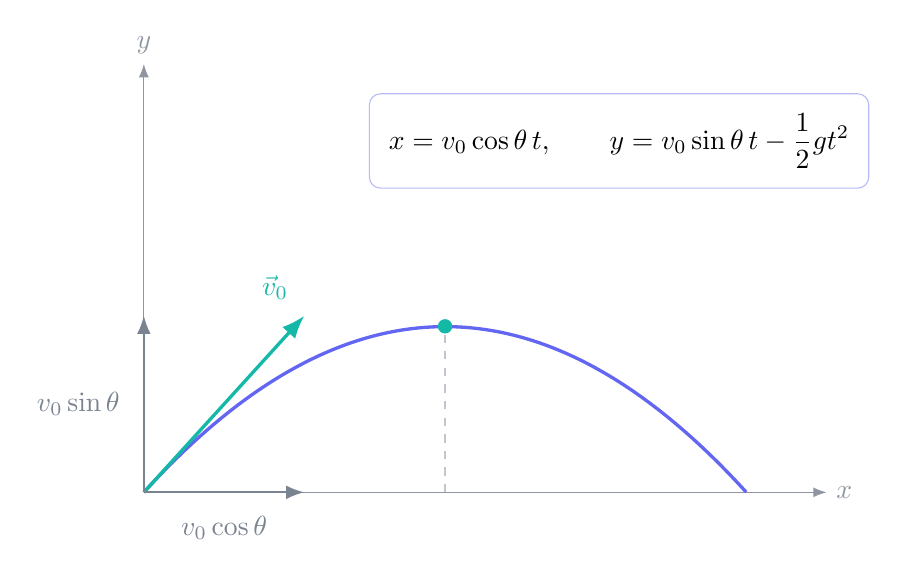
\begin{tikzpicture}[font=\sffamily,>=Latex,x=.85cm,y=.85cm]
  \draw[->,ink!55] (0,0)--(10.2,0) node[right] {$x$};
  \draw[->,ink!55] (0,0)--(0,6.4) node[above] {$y$};
  \draw[very thick,nebula,domain=0:9,samples=120,smooth] plot(\x,{1.1*\x-.1222*\x*\x});
  \draw[->,very thick,spark] (0,0)--(2.4,2.64) node[above left=2pt] {$\vec v_0$};
  \draw[->,thick,ink!65] (0,0)--(2.4,0) node[midway,below=5pt] {$v_0\cos\theta$};
  \draw[->,thick,ink!65] (0,0)--(0,2.64) node[midway,left=5pt] {$v_0\sin\theta$};
  \draw[dashed,ink!30] (4.5,0)--(4.5,2.48);
  \fill[spark] (4.5,2.48) circle (2.6pt);
  \node[draw=nebula!45,rounded corners=4pt,fill=white,inner sep=7pt] at (7.1,5.25)
    {$\displaystyle x=v_0\cos\theta\,t,\qquad y=v_0\sin\theta\,t-\frac12gt^2$};
\end{tikzpicture}
\end{document}
